\begin{center}
    \vspace*{1.5cm}
    {\fontsize{20}{20}\textbf{Ölvisor}}\\
    \vspace{0.7cm}
    {\fontsize{12}{12}\textit{Om jästen själv får välja}}
\end{center}
\addtocwithheader{Ölvisor}  % Add entry to TOC and set header\noBackground
\noBackground

\newpage
\noBackground


\begin{textblock*}{3cm}(6cm,9cm) % {width}(x, y)
    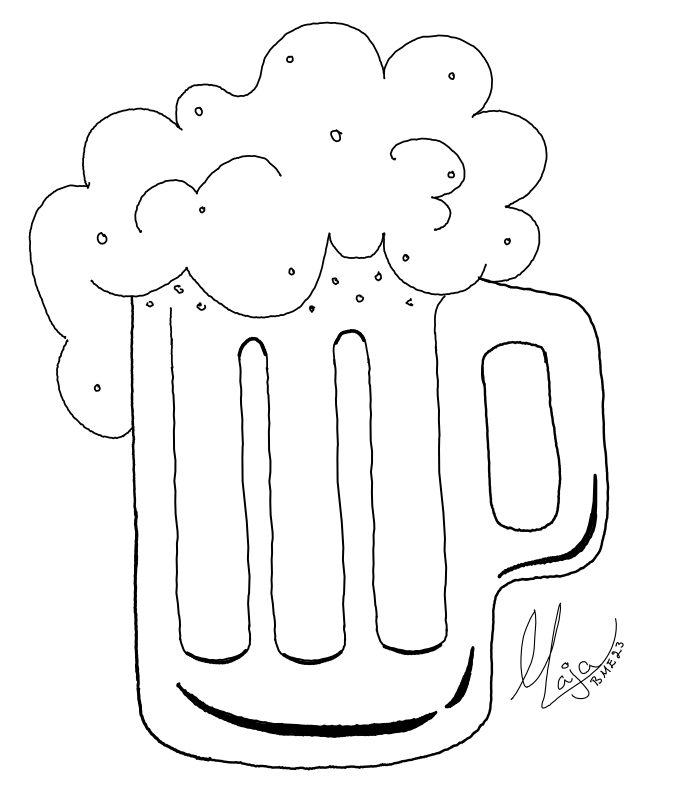
\includegraphics[width=3.5cm]{./bilder/majas-bilder/olglas.png}
\end{textblock*}


\subsection*{Ode till ölet} 
\index[alfa]{Ode till ölet}
\index[anfa]{Tu tu tu Tuborg}
\songinfo{Mel: Trampa på gasen}

\begin{parse lines}[\noindent]{#1\\}
    Tu tu tu Tuborg
    och ca ca ca Carlsberg
    det är den bästa
    pi pi pi pilsnern som jag vet

    Tu tu tu Carlsberg
    och ca ca ca Tuborg
    det är det bästa
    pi pi pi ölet som jag vet

    Tu tu tu Ölberg
    och ca ca ca Pilsborg
    det är den bästa
    pi pi pi biran som jag vet

    Tu ca pi Ölsner
    och pi tu ca bira
    det är den bästa
    ca pi tu lering som jag gjort
\end{parse lines}

\newpage
\resetBackground

\begin{textblock*}{3cm}(5.5cm,4.5cm) % {width}(x, y)
%    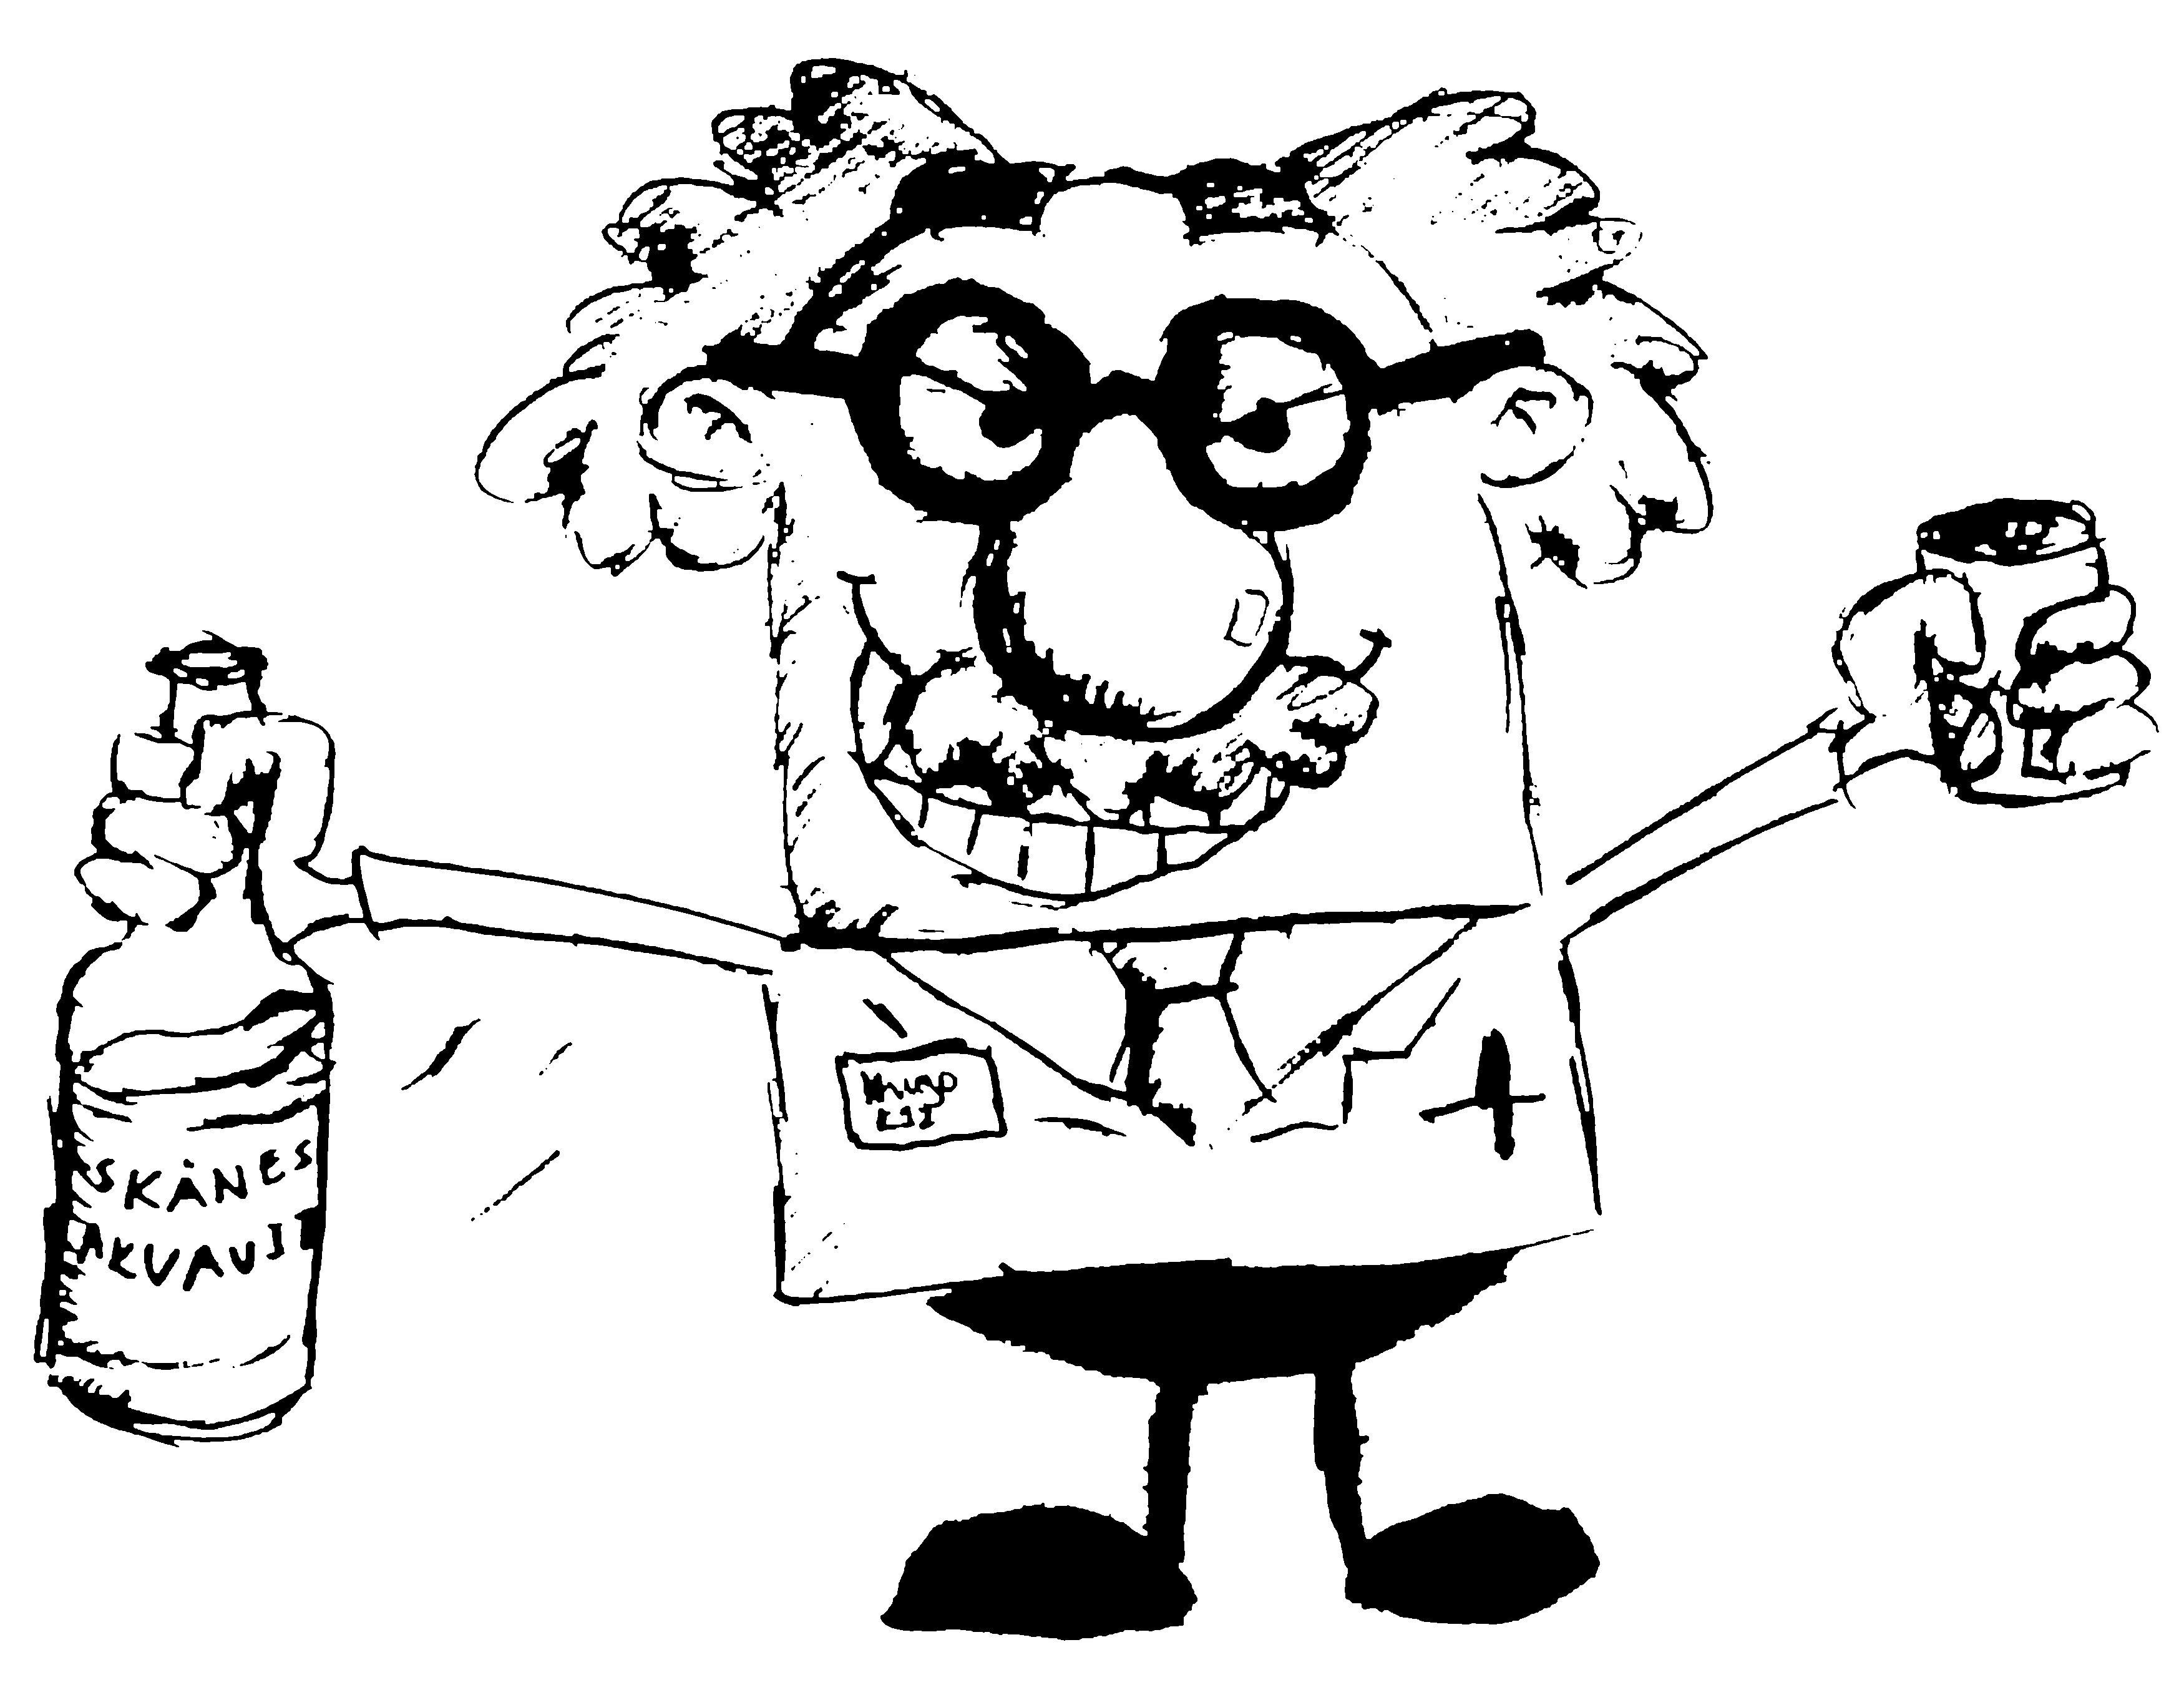
\includegraphics[width=4.9cm]{./bilder/GalenVetenskapsmanTransparent.png}
    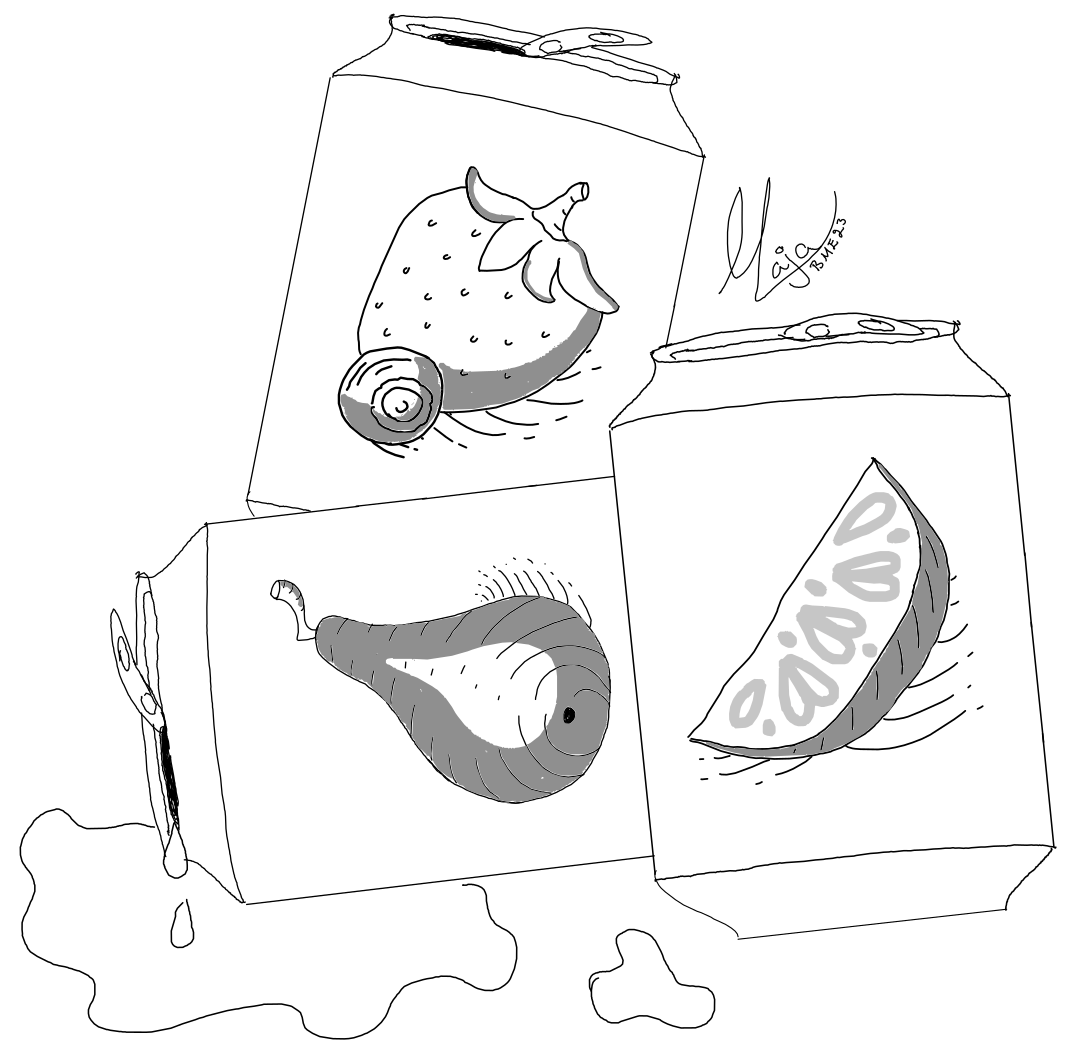
\includegraphics[width=4cm]{./bilder/majas-bilder/en_sot_dryck.png}
\end{textblock*}

\subsection*{Om en söt dryck} 
\index[alfa]{Om en söt dryck}
\index[anfa]{Man é ej dum för att man dricker cider}
\songinfo{Mel: Jag fångade en räv idag\\
Text: Erik Johanneson F99}

\begin{parse lines}[\noindent]{#1\\}
    Jag dricker gärna öl och vin
    till sillen tar jag nubben
    och kanske till och med en shot
    när jag har gått till klubben.

    Men drycken som jag helst vill ha
    den har så friska lukter
    den är dessutom ren och klar
    och smakar utav frukter

    Hå hum, man är ej dum
    för att man dricker cider
    Även om, det finnes dom
    som utav smaken lider

    Det skummar upp i glaset när
    man har hällt upp en cider
    det smakar både sött och gott
    när den i halsen glider

    Det kan vá både söt och torr
    av tranbär eller fläder
    av plommon och det finns nån sort
    som smakar gamla kläder

    Hå hum, man är ej dum...
\end{parse lines}

\vissteduatt{Visste du att en av Sveriges första datorer byggdes och drevs i Lund?\\Den hetter SMIL, en förkortning av SifferMaskinen I Lund.}

\newpage

\subsection*{Oralöl} 
\index[alfa]{Oralöl}
\index[anfa]{Min vän Kal, är Dual}
\songinfo{Mel: B.L.O.S.S.A\\
Lundakarnevalen 2006}

\begin{parse lines}[\noindent]{#1\\}
    Min vän Kal, är Dual
    Hans anal, är verbal
    Så när Kal, håller tal,
    kan han halsa pilsner!
\end{parse lines}

\subsection*{Importvisan} 
\index[alfa]{Importvisan}
\index[anfa]{T-U-B-O-R-G}
\songinfo{Mel: B.L.O.S.S.A\\
Lundakarnevalen 2022}

\begin{parse lines}[\noindent]{#1\\}
    T-U-B-O-R-G
    T-U-B-O-R-G
    T-U-B-O-R-G
    Den är importerad!
\end{parse lines}

\subsection*{Öl, öl, öl i glas} 
\index[alfa]{Öl, öl, öl i glas}
\index[anfa]{Öl, öl, öl i glas}
\songinfo{Mel: Row your boat}

\begin{parse lines}[\noindent]{#1\\}
    Öl, öl, öl i glas eller i butelj
    Skummande, skummande,
    skummande, skummande
    Ta en klunk och svälj
\end{parse lines}


\vissteduatt{Visste du att E-sektionens huvudserver heter EMIL,
\\en förkorning av E-sektionens Magnifika Internet-Låda.}

\newpage

\subsection*{Strejk på Pripps} 
\index[alfa]{Strejk på Pripps}
\index[anfa]{Inatt jag drömde något som...}
\songinfo{Mel: I natt jag drömde}

\begin{parse lines}[\noindent]{#1\\}
    Inatt jag drömde något som,
    jag aldrig drömt förut
    Jag drömde det var strejk på Pripps
    och alla ölen var slut
    Jag drömde om en jättesal
    där ölen stod på rad
    Jag drack sådär en femton öl
    och reste mig och sa:
    "Man kan ha roligt utan sprit,
    men det är dumt att chansa!"
\end{parse lines}


\subsection*{Ont i huvudet} 
\index[alfa]{Ont i huvudet}
\index[anfa]{Om du har ont i huvet}
\songinfo{Mel: Jag har en gammal faster}

\begin{parse lines}[\noindent]{#1\\}
    Om du har ont i huvet
    när du vaknar någon da'
    så häll en öl i håret
    och låt den stå och dra

    Och känns det inte bättre
    så skyll inte på oss,
    Att hälla öl i huvet
    är inte smart förstås
\end{parse lines}

\newpage
\noBackground

\begin{textblock*}{3cm}(4cm,8.8cm) % {width}(x, y)
    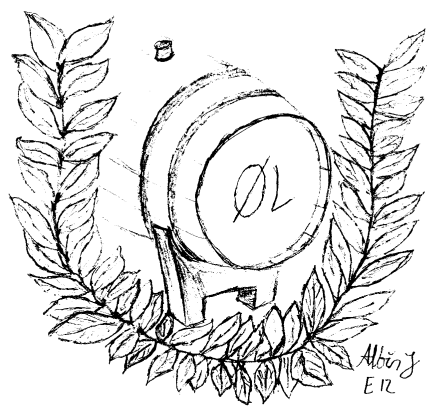
\includegraphics[width=5.0cm]{./bilder/bild_1_tunna_ol.png}
\end{textblock*}

\subsection*{Var nöjd med ölen} 
\index[alfa]{Var nöjd med ölen}
\index[anfa]{Var nöjd med allt som ölen ger}
\songinfo{Mel: Var nöjd med allt vad livet ger}

\begin{parse lines}[\noindent]{#1\\}
    Var nöjd med allt som ölen ger
    och även om du dubbelt ser
    Glöm bort bekymmer sorger och besvär
    Var glad och nöjd för vet du vad
    en folköl gör ju ingen glad
    Var nöjd med ölen som vi dricker här
\end{parse lines}

\subsection*{Ölkanon} 
\index[alfa]{Ölkanon}
\index[anfa]{Drick, drick, drick din öl}
\songinfo{Mel: Row your boat\\
Lundakarnevalen 2002}

\begin{parse lines}[\noindent]{#1\\}
    Drick, drick, drick din öl,
    låt den rinna ner.
    Kan du sen kraxa,
    “en laxask med slasktratt”
    så får du dricka fler
\end{parse lines}

\vissteduatt{Visste du att låten heter Ölkanon, dvs. man ska sjunga den i kanon \\
och inte att det är en artilleripjäs med öl.}
\newpage
\resetBackground

\subsection*{Min pilsner} 
\index[alfa]{Min pilsner}
\index[anfa]{Min pilsner}
\songinfo{Mel: My Bonnie}

\begin{parse lines}[\noindent]{#1\\}
    Min pilsner skall svalka min tunga
    Min pilsner skall duscha min gom
    Min pilsner skall få mig att sjunga,
    om jag ser att flaskan är tom:

    PILSNER! PILSNER!
    Hämta en pilsner till mig, till mig
    PILSNER! PILSNER!
    Hämta en pilsner till mig!
\end{parse lines}


\subsection*{Min trasa} 
\index[alfa]{Min trasa}
\index[anfa]{Min trasa}
\songinfo{Mel: My Bonnie\\
Text: Kewin Erichsen E11, Henrik Fryklund E13}

\begin{parse lines}[\noindent]{#1\\}
    Min pilsner har spillts ut på bordet
    Min pilsner har lämnat mitt glas
    Min pilsner har sölat min ovve
    och nu blir grannen indignerad på mig

    Trasa! Trasa!
    Hämta en trasa till mig, till mig
    Trasa! Trasa!
    Hämta en ny pilsner till mig!
\end{parse lines}

\vissteduatt{Visste du att Min Trasa skrevs för att fylla ut sidan?}

\newpage

\subsection*{Då ölen är kall} 
\index[alfa]{Då ölen är kall}
\index[anfa]{Det är nu som ölen är kall}
\songinfo{Mel: Gabriellas sång\\ Text: Axel Lundholm E12, Hugo Hjertén E12}

\noindent Det är nu som ölen är kall, \textbf{bam bam}\\
\begin{parse lines}[\noindent]{#1\\}
    Den har väntat på mig i kylen
    Sakteligen jag rör mig dit
    För att stilla min bittra törst
\end{parse lines}
\noindent Tidigare samma dag, \textbf{bam bam}\\
\begin{parse lines}[\noindent]{#1\\}
    Jag begav mig mot systemet
    Jag var där strax innan tre
    Men systemet det stängde två!
    
    Jag vill hälla öl i strupen
    Humle mot min gom
    Men kylen den står tom
    Ölen som jag hoppats på 
    Är blott en fakking illusion
    
    …Men!
    Jag har faktiskt ännu än öl i min kyl!
\end{parse lines}

\vissteduatt{Visste du att denna sång görs bäst med en kyld oöppnad\\och förväntansfylld öl?}


\newpage